\documentclass{beamer}
\usepackage[T1]{fontenc}
\usepackage[utf8]{inputenc}
\usepackage[german]{babel}
\usepackage{pdfpages}
\usepackage{amssymb}
\usepackage{enumerate}
\usepackage{array}
\usepackage{lmodern}
\usepackage{url}
\usepackage{hyperref}
\usepackage[all]{xy}
\usepackage[export]{adjustbox}
\usepackage{subcaption}
\usepackage{listings}
\usepackage{graphicx}
\graphicspath{{./img/}}

%Farbschema
\definecolor{tuerkis}{rgb}{0.0, 0.65, 0.76}
\definecolor{weiss}{rgb}{1.0,1.0,1.0}
\definecolor{gruen}{rgb}{0.22, 0.74, 0.07}

\usetheme{metropolis}
%\usecolortheme{whale}
\setbeamercolor{progress bar}{fg=gruen,bg=gruen}
\setbeamercolor{frametitle}{bg = gruen}
\setbeamercolor{background canvas}{bg = weiss}
\setbeamercolor{footline}{fg=gray}
\setbeamerfont{page number in head/foot}{size=\scriptsize}
\setbeamercolor{title}{fg = black}
\setbeamertemplate{frame footer}{ \insertlogo{
\includegraphics[width=0.1\textwidth]{aegis_logo_with_name.pdf}} \hfill  \insertsection}
\lstset{frame=single}

%\logo{
\includegraphics[width=.1\textwidth]{aegis_logo_with_name.pdf}\hspace*{.05\paperwidth}}
%\logo{
\includegraphics[width=.1\textwidth]{img/aegis_logo_with_name.pdf}}
\newcommand\pipeline{\center 
\includegraphics[width=0.6\linewidth]{grobentwurf/packet_diagram_pipeline.png}}

%Information to be included in the title page:
\title[Abwehr von Denial-of-Service-Angriffen durch effiziente User-Space Paketverarbeitung: AEGIS]{Abwehr von Denial-of-Service-Angriffen durch effiziente User-Space Paketverarbeitung: AEGIS}
\subtitle{Review für die Implementierungsphase}
\institute{Technische Universität Ilmenau}
\date{24.06.2021}

\begin{document}

\begin{frame}
    \maketitle % Automatically created using the information in the commands above
\end{frame}

\begin{frame}{Aufgabenstellung}
    \center
    
\includegraphics[width=0.3\textwidth]{dpdk_logo.png}
    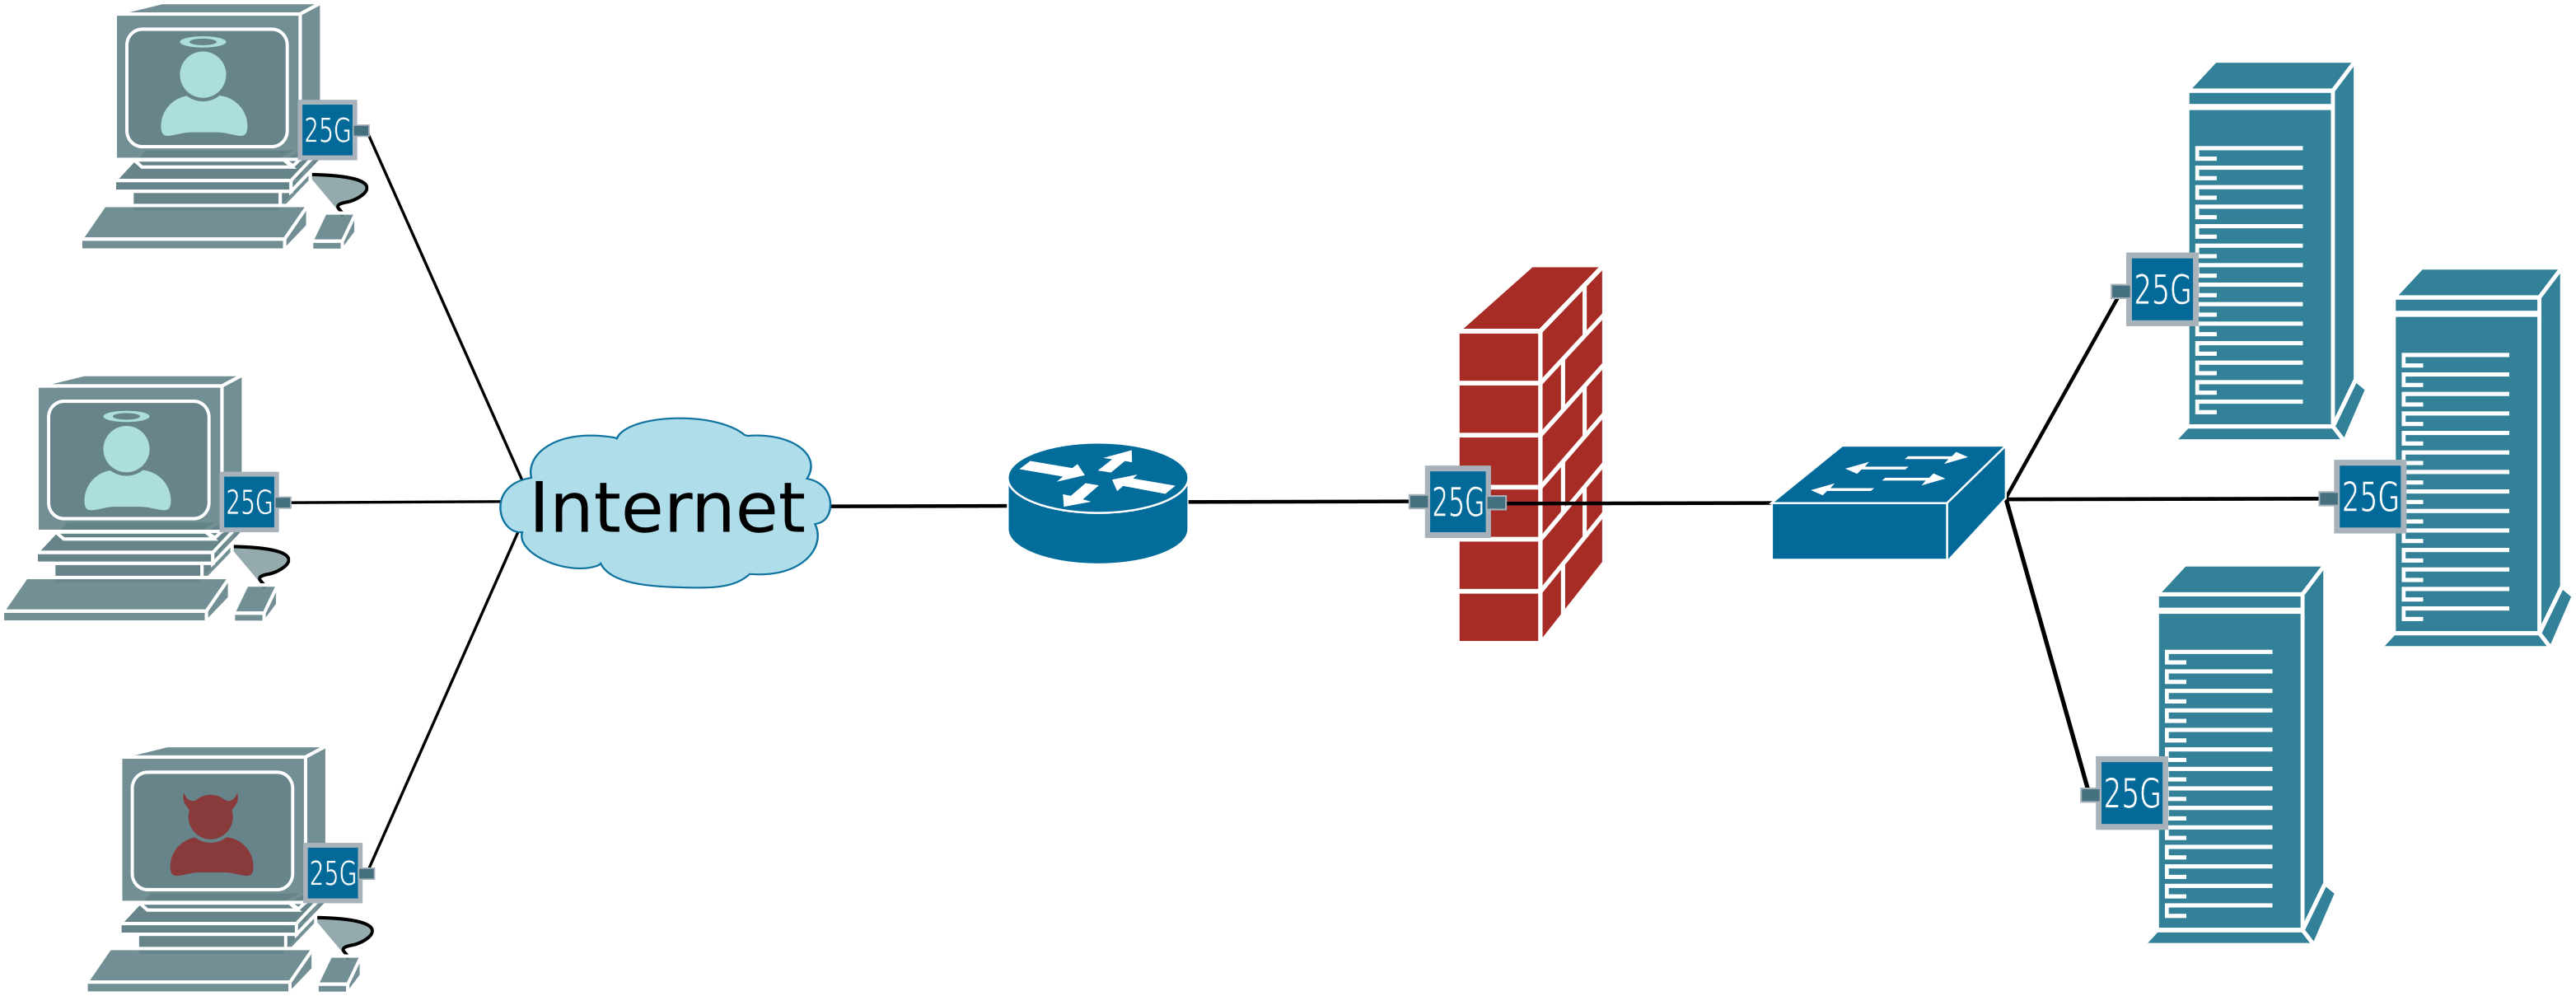
\includegraphics[width=\textwidth]{Netzwerkplan-Real.png}
    \center
    Abwehrsystem gegen DoS-Angriffe
\end{frame}

\begin{frame}{Aufgabenstellung}
    \begin{itemize}
        \item Die Software soll mehrere Varianten von Attacken abwehren
        \item Nur eine davon ist für diesen Vortrag relevant:
    \end{itemize}
    \center
    \textbf{SYN-Flood-Attacke}
    \begin{figure}[h!]
        \includegraphics[width=0.5\textwidth]{SYN-FLOOD.png}
    \end{figure}
\end{frame}

\begin{frame}{Gliederung}
    \begin{enumerate}
        \item \textbf{Grobentwurf}
        \item \textbf{Feinentwurf}
              \begin{enumerate}
                  \item Komponente: NicManagement
                  \item Komponente: PacketDissection
                  \item Komponente: Inspection
                  \item Komponente: Treatment
                  \item Einsatz von mehreren Threads
                  \item Alternative Entwürfe
              \end{enumerate}
        \item \textbf{Entwurfsmuster}
        \item \textbf{Stand des Projekts}
        \item \textbf{Ausblick}
    \end{enumerate}
\end{frame}

% =====   G R O B E N T W U R F   ===== %
\begin{frame}{Grobentwurf}
    \begin{center}
    %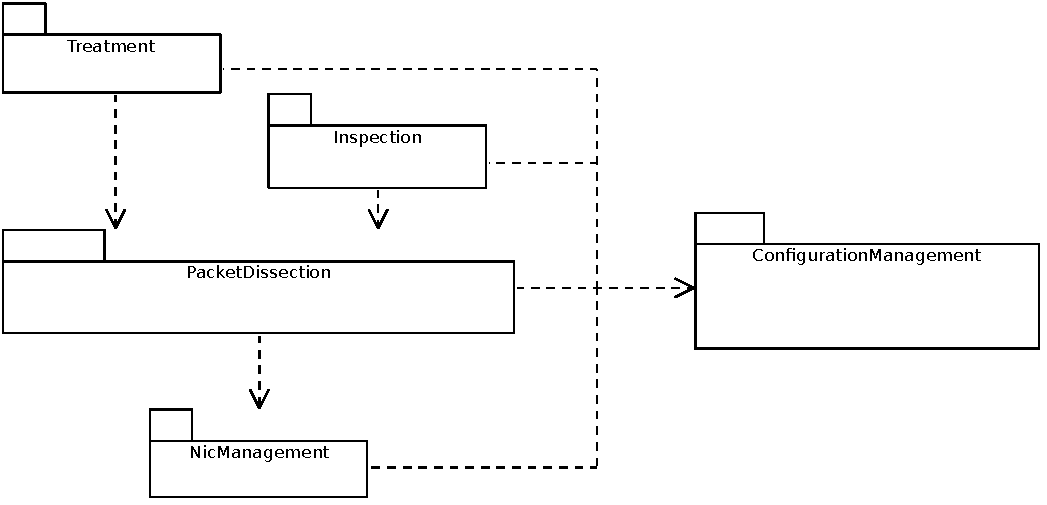
\includegraphics[width=\linewidth]{grobentwurf/packet_diagram.pdf}
    \end{center}
\end{frame}

\begin{frame}{Grobentwurf}
    \begin{center}
    %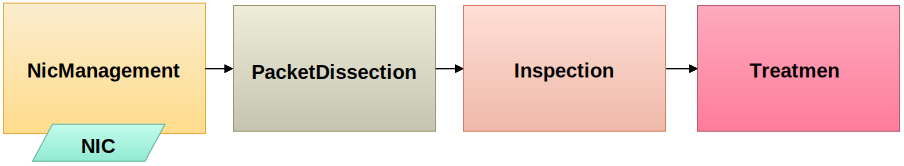
\includegraphics[width=0.95\linewidth]{roadmap/roadmap2.pdf}
    Die Architektur folgt dem Pipeline-Modell.
    \end{center}
\end{frame}

% =====   F E I N E N T W U R F   ===== %
\begin{frame}{Feinentwurf}
    %\includegraphics[width=\textwidth]{roadmap/roadmap2_1.pdf}
\end{frame}

\begin{frame}{Feinentwurf: NicManagement}
    \begin{figure}
        
\includegraphics[width=0.3\textwidth]{dpdk_logo.png}
        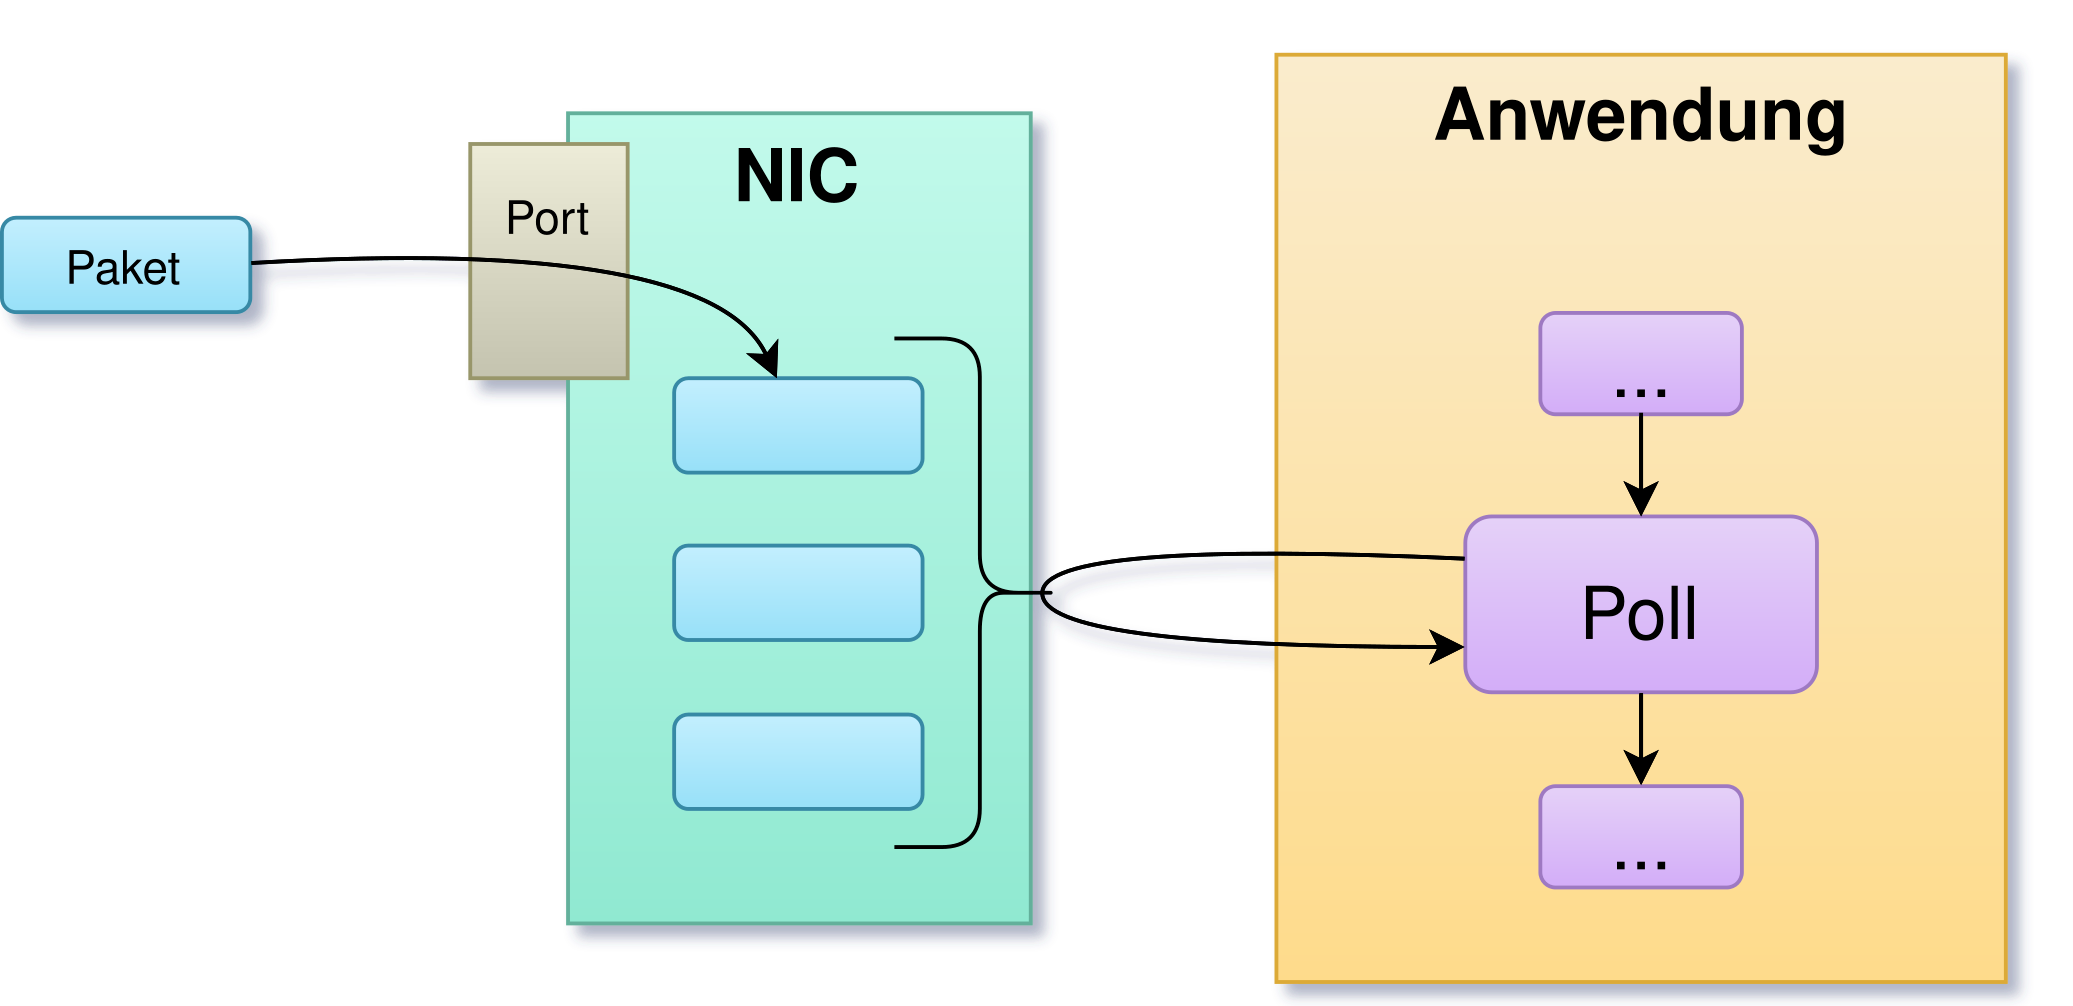
\includegraphics[width=\linewidth]{polling.png}
        \center
        effizient Pakete von der NIC bekommen: Polling
    \end{figure}
\end{frame}

\begin{frame}{Feinentwurf: PacketDissection}
    %\includegraphics[width=\textwidth]{roadmap/roadmap2_2.pdf}
\end{frame}

\begin{frame}{Feinentwurf: PacketDissection}
    %\includegraphics[width=\textwidth]{roadmap/roadmap2_2.pdf}
    \begin{itemize}
        \item extrahiert Informationen aus den Paketen
        \item stellt diese für die folgenden Komponenten bereit
    \end{itemize}
\end{frame}

\begin{frame}{Feinentwurf: Inspection}
    %\includegraphics[width=\textwidth]{roadmap/roadmap2_3.pdf}
\end{frame}

\begin{frame}{Feinentwurf: Inspection}
    \begin{minipage}[h]{0.45\textwidth}
        \begin{figure}[h!]
            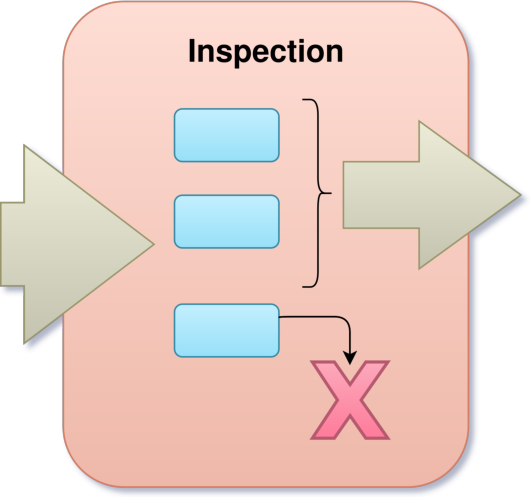
\includegraphics[width=\textwidth, center]{inspection.pdf}
        \end{figure}
    \end{minipage}
    \hfill
    \begin{minipage}[h]{0.45\textwidth}
        \begin{itemize}
            \item Klasse Analyzer
            \item Filterung aller Pakete der Netzwerkprotokolle UDP, TCP, ICMP
            \item Abwehr von SYN-FIN-Angriffen
        \end{itemize}
    \end{minipage}
\end{frame}

\begin{frame}{Feinentwurf: Inspection}
    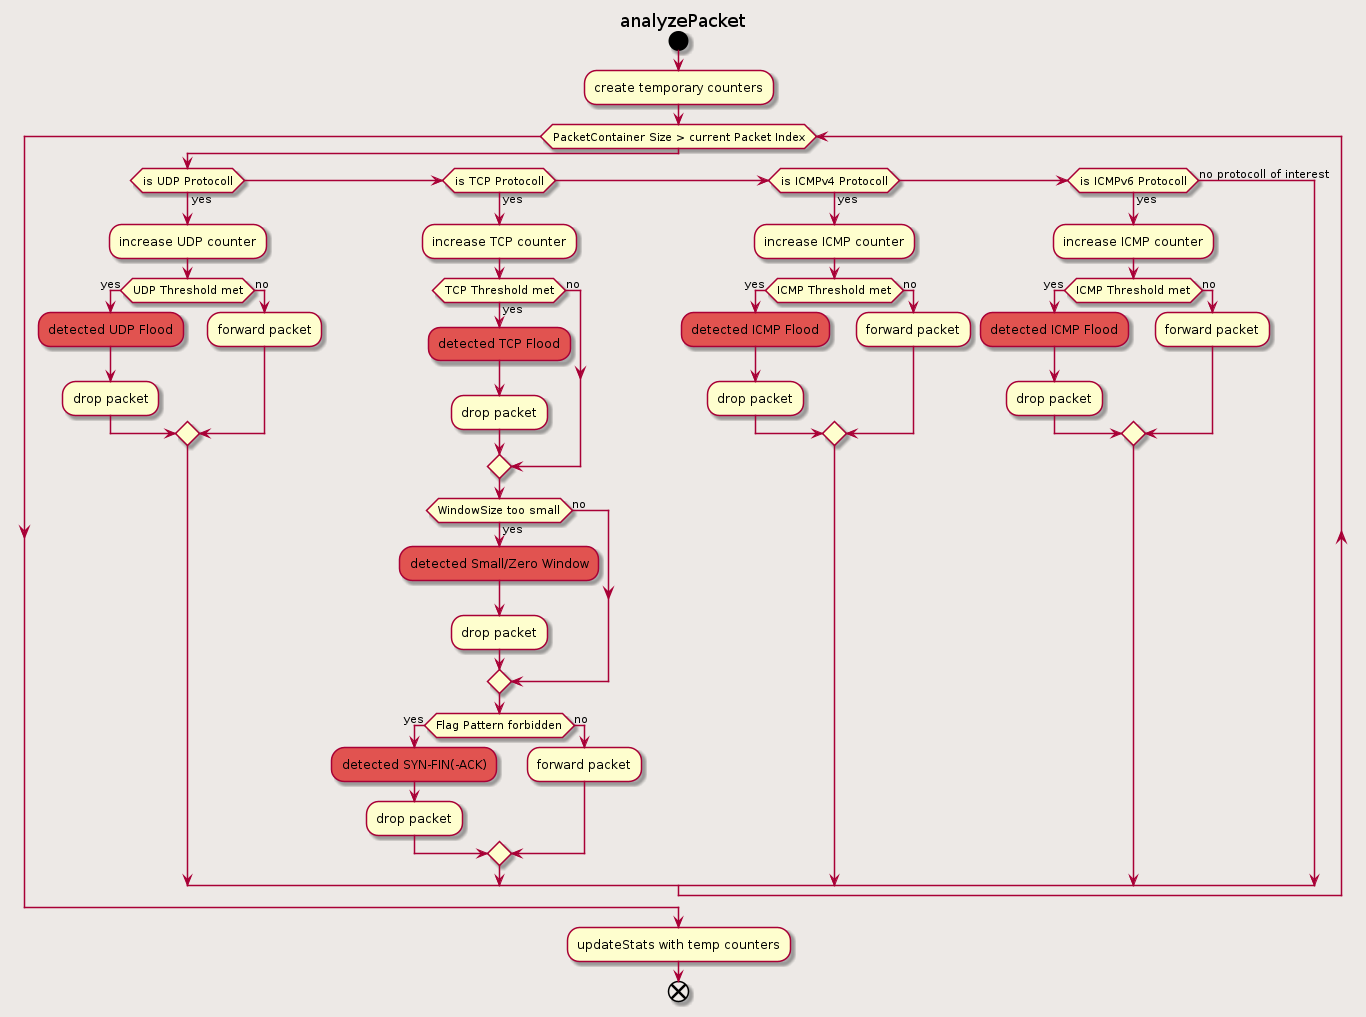
\includegraphics[width=\textwidth, center]{analyzerDiagram.png}
\end{frame}

\begin{frame}{Feinentwurf: Treatment}
    %\includegraphics[width=\textwidth]{roadmap/roadmap2_4.pdf}
\end{frame}

\begin{frame}{Feinentwurf: Treatment}
    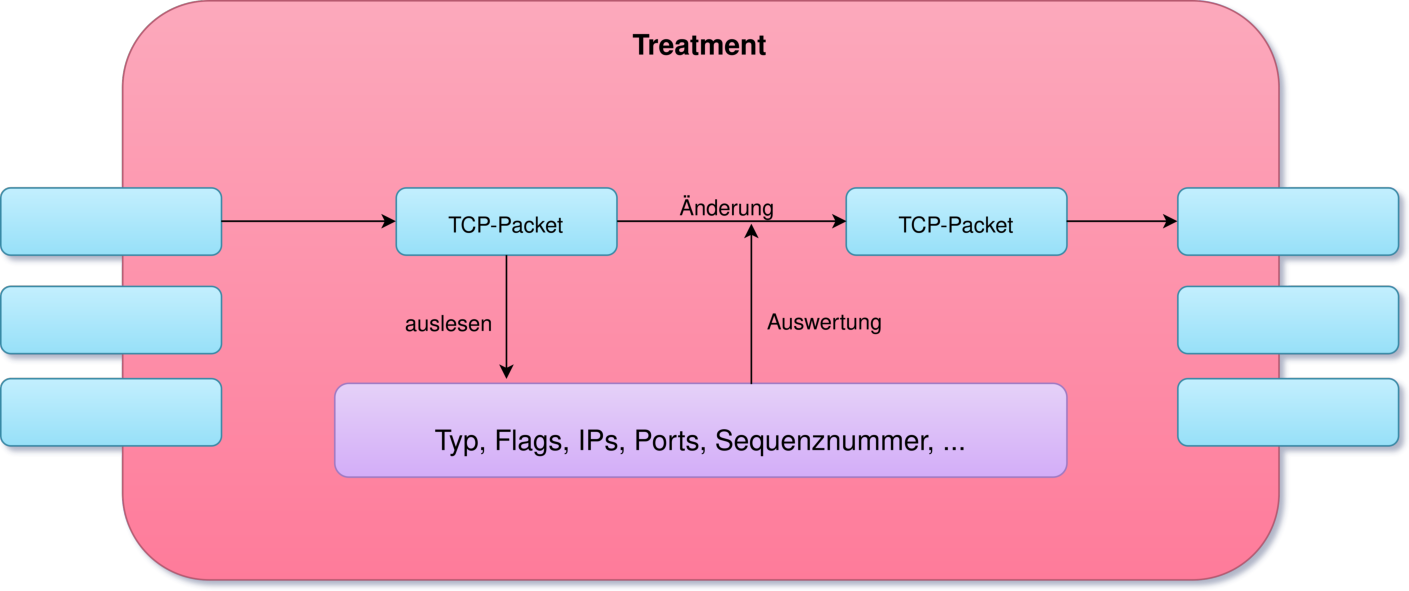
\includegraphics[width=\textwidth, center]{Treatment_ohne_Container_mit_Schatten.pdf}
\end{frame}

\begin{frame}{Feinentwurf: Treatment}
    \begin{minipage}[h]{0.45\textwidth}
        \includegraphics[width=\textwidth, center]{SYN-FLOOD.png}
    \end{minipage}
    \hfill
    \begin{minipage}[h]{0.45\textwidth}
        \begin{itemize}
            \item SYN-Flood-Abwehr mit SYN-Cookies
            \item keine Reservierung von Ressourcen beim Aufbau
        \end{itemize}
    \end{minipage}
\end{frame}

\begin{frame}{Feinentwurf: Treatment}
    \begin{minipage}[h]{0.5\textwidth}
        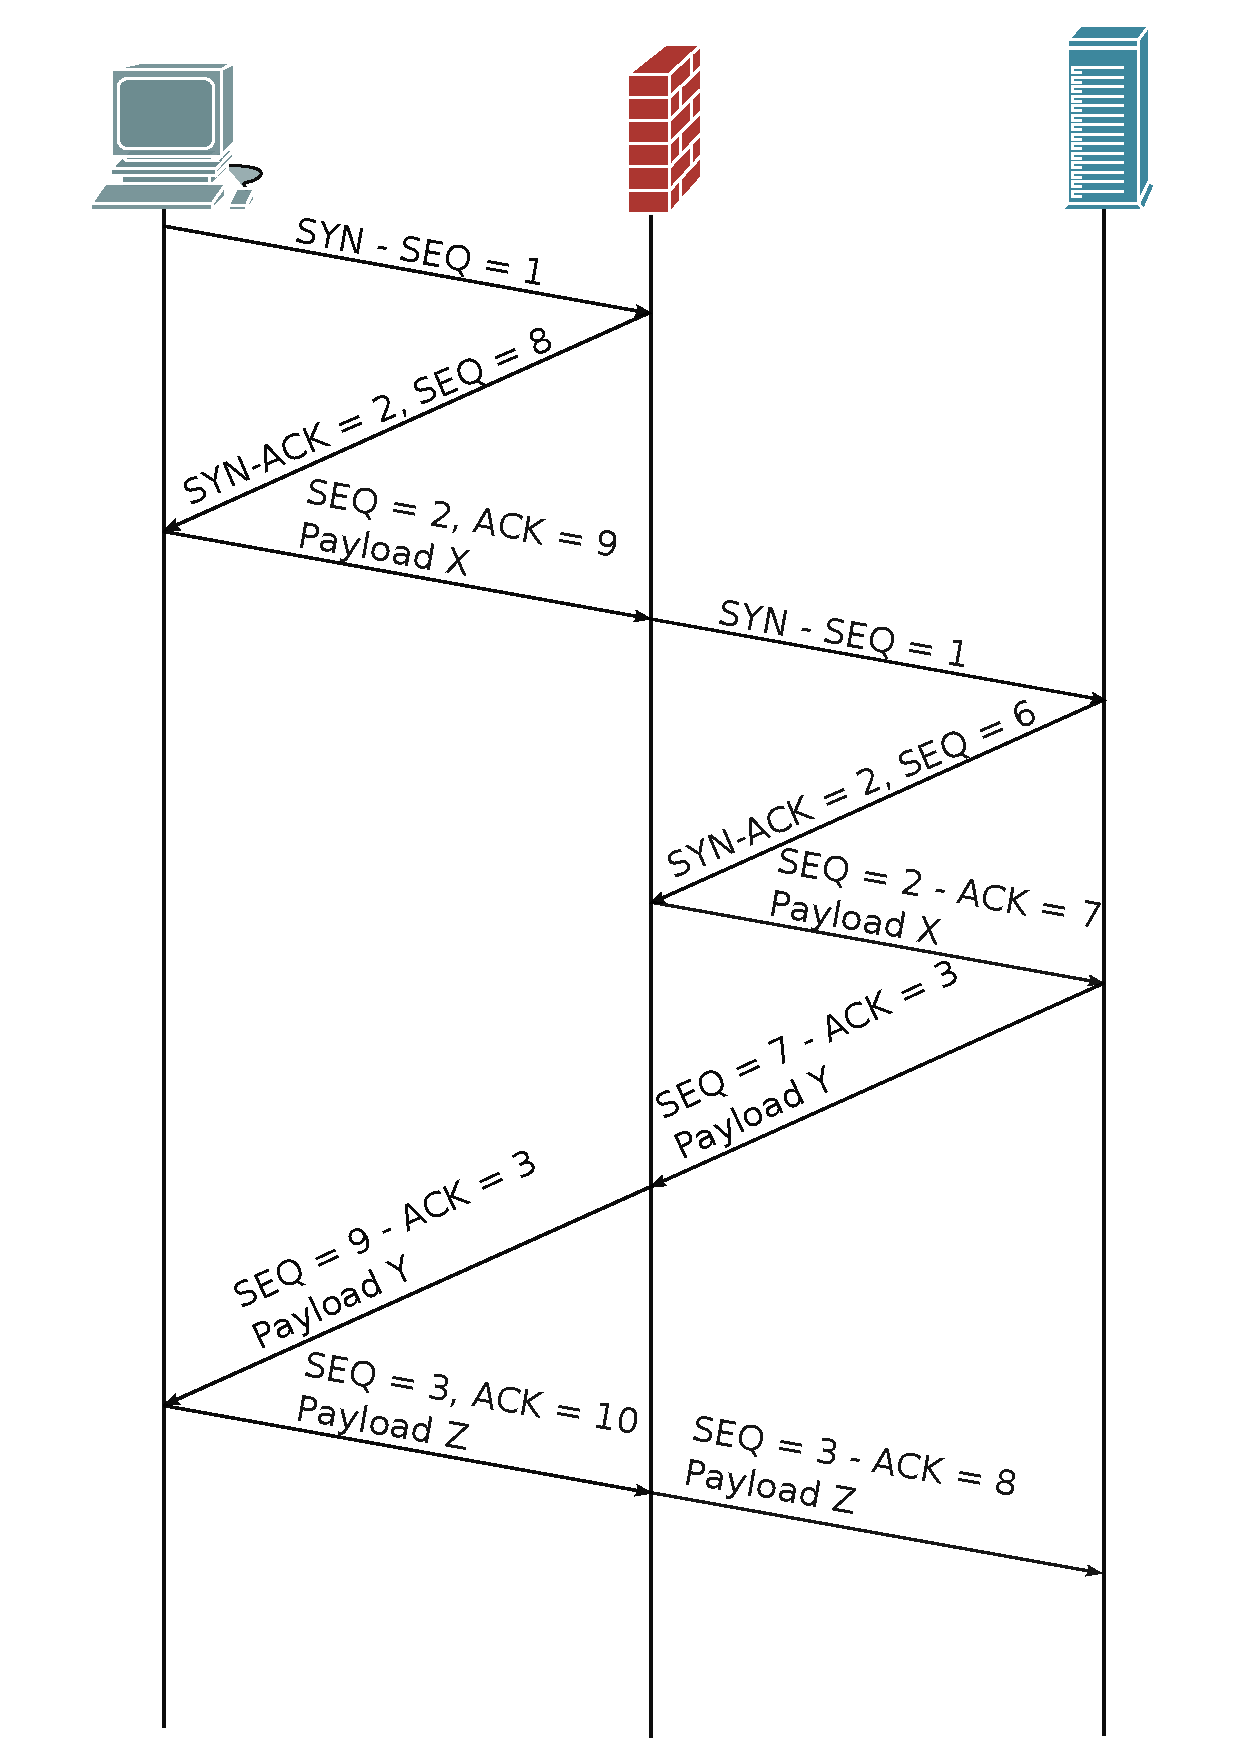
\includegraphics[width=\textwidth, center]{splicing.pdf}
    \end{minipage}
    \hfill
    \begin{minipage}[h]{0.45\textwidth}
        \begin{itemize}
            \item TCP-Proxy
            \item Middle-Box als Vermittler
        \end{itemize}
    \end{minipage}
\end{frame}

\begin{frame}[fragile]
    \frametitle{Implementierung Treatment}
    {\footnotesize
        \begin{lstlisting}
Treatment::treat_packtes(){
  for packet in packet_to_inside{
    if(packet.get_type() == packet_type_tcp){
      flags = packet.get_flags();
        if(flags.is_pure_syn()){
          syn_cookie = calc_cookie(connection_data);
          reply_packet = get_empty_packet_to_outside;
          reply_packet.fill(connection_data,syn_cookie);		
        }
        else if(...){...}
        ...		
    } 	
  }			
}
		\end{lstlisting}
    }
\end{frame}

\begin{frame}{Feinentwurf: Einsatz von Threads}
    \begin{itemize}
        \item eine Pipeline \(\rightarrow\) nur ein Thread nötig
    \end{itemize}
    %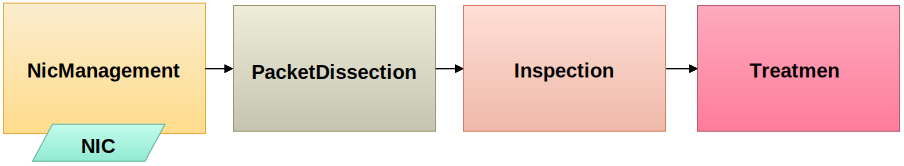
\includegraphics[width=\linewidth]{roadmap/roadmap2.pdf}
\end{frame}

\begin{frame}{Feinentwurf: Einsatz von Threads}
    \begin{itemize}
        \item Wünsche für Effizienz:
              \begin{itemize}
                  \item mehrere Threads parallel
                  \item gleichmäßig ausgelastet
                  \item keine Kommunikation
              \end{itemize}
    \end{itemize}
    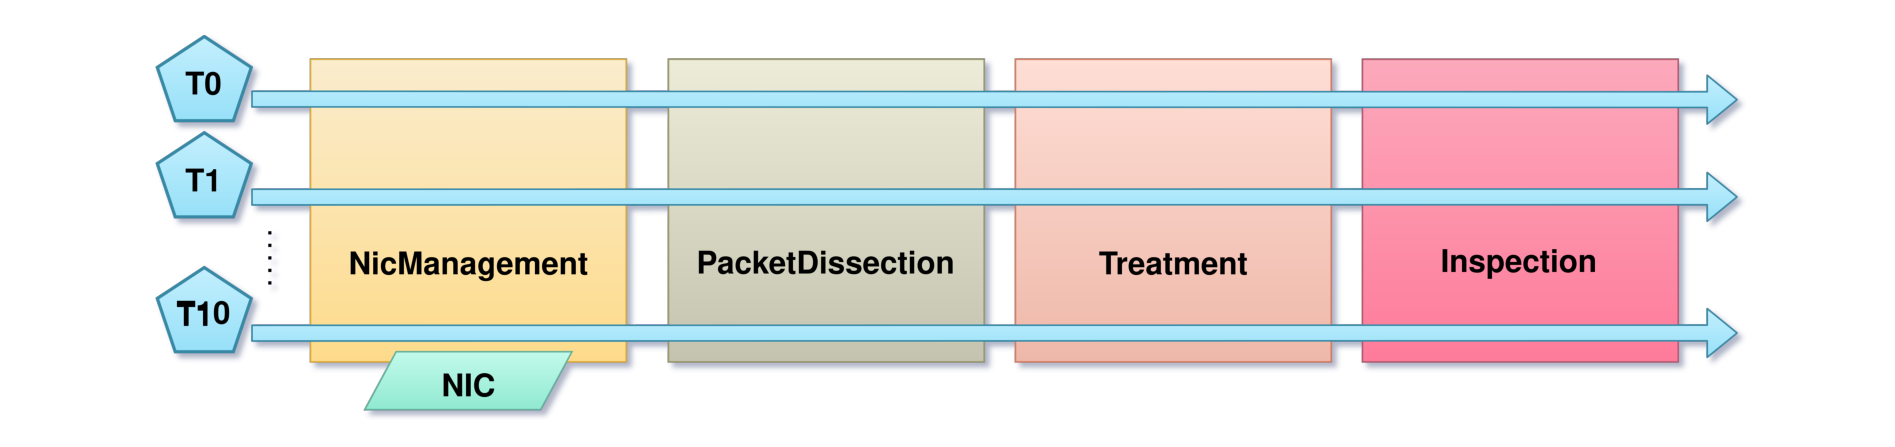
\includegraphics[width=\linewidth]{multithreading2.pdf}
\end{frame}

\begin{frame}{Feinentwurf: Einsatz von Threads}
    \begin{itemize}
        \item Pakete aufgeteilt durch ,,RSS'' (Receive Side Scaling)
              \begin{itemize}
                  \item realisiert durch Hashing
                  \item Schlüssel: \texttt{[Src-IP; Dst-IP; Src-Port; Dst-Port]}
              \end{itemize}
    \end{itemize}
    \begin{figure}
        \center
        %\includegraphics[width=0.8\linewidth]{rss/rss.pdf}
    \end{figure}
    \begin{itemize}
        \item \textbf{gleichmäßige Auslastung} (wegen Hashing)
    \end{itemize}
\end{frame}

\begin{frame}{Feinentwurf: Einsatz von Threads}
    \begin{itemize}
        \item Problem: Verschiedene Zuordnung je Seite
              \begin{itemize}
                  \item[\(\rightarrow\)] Inter-Thread-Kommunikation nötig!
              \end{itemize}
    \end{itemize}
    \begin{figure}
        \center
        %\includegraphics[width=\linewidth]{rss/sym_rss_solution.pdf}
    \end{figure}
\end{frame}

\begin{frame}{Feinentwurf: Einsatz von Threads}
    \begin{itemize}
        \item Lösung: ,,Symmetric RSS''
              \begin{itemize}
                  \item \texttt{[\textbf{Src-IP}; \textit{Dst-IP}]} \(\equiv\) \texttt{[\textit{Dst-IP}; \textbf{Src-IP}]}
                  \item[\(\rightarrow\)] \textbf{keine Inter-Thread-Kommunikation nötig}
              \end{itemize}
    \end{itemize}
    \begin{figure}
        \center
        %\includegraphics[width=\linewidth]{rss/sym_rss_problem.pdf}
    \end{figure}
\end{frame}

\begin{frame}{Feinentwurf: Alternative Entwürfe}
    % Alternativen (Implementierungsentscheidungen, Grobentwurfsänderung)
    \begin{figure}
        \center
        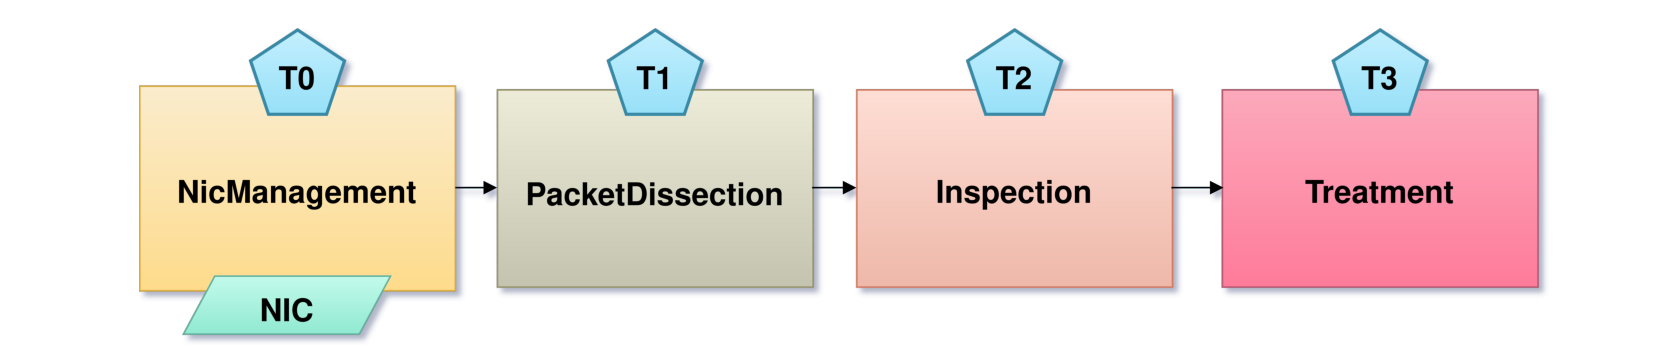
\includegraphics[width=\textwidth]{multithreading_old.pdf}
    \end{figure}
    \begin{itemize}
        \item alternativ: ein Thread pro Komponente
        \item Nachteil: zu viel Inter-Thread-Kommunikation
    \end{itemize}
\end{frame}

\begin{frame}{Entwurfsmuster}
    \begin{minipage}[h]{0.45\textwidth}
        \begin{figure}[h!]
            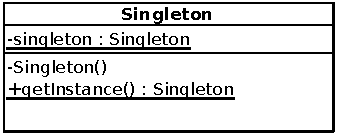
\includegraphics[width=\textwidth]{singleton.pdf}
        \end{figure}
    \end{minipage}
    \hfill
    \begin{minipage}[h]{0.45\textwidth}
        \begin{itemize}
            \item Erzeugungsmuster
            \item Nur ein Objekt dieser Klasse
            \item Globale Informationsbereitstellung
            \item Verwendung im Configurator
        \end{itemize}
    \end{minipage}
\end{frame}

\begin{frame}{Was AEGIS bisher kann}
    \begin{minipage}[h]{\textwidth}
        \center
        \begin{minipage}[h]{0.5\textwidth}
            \center
            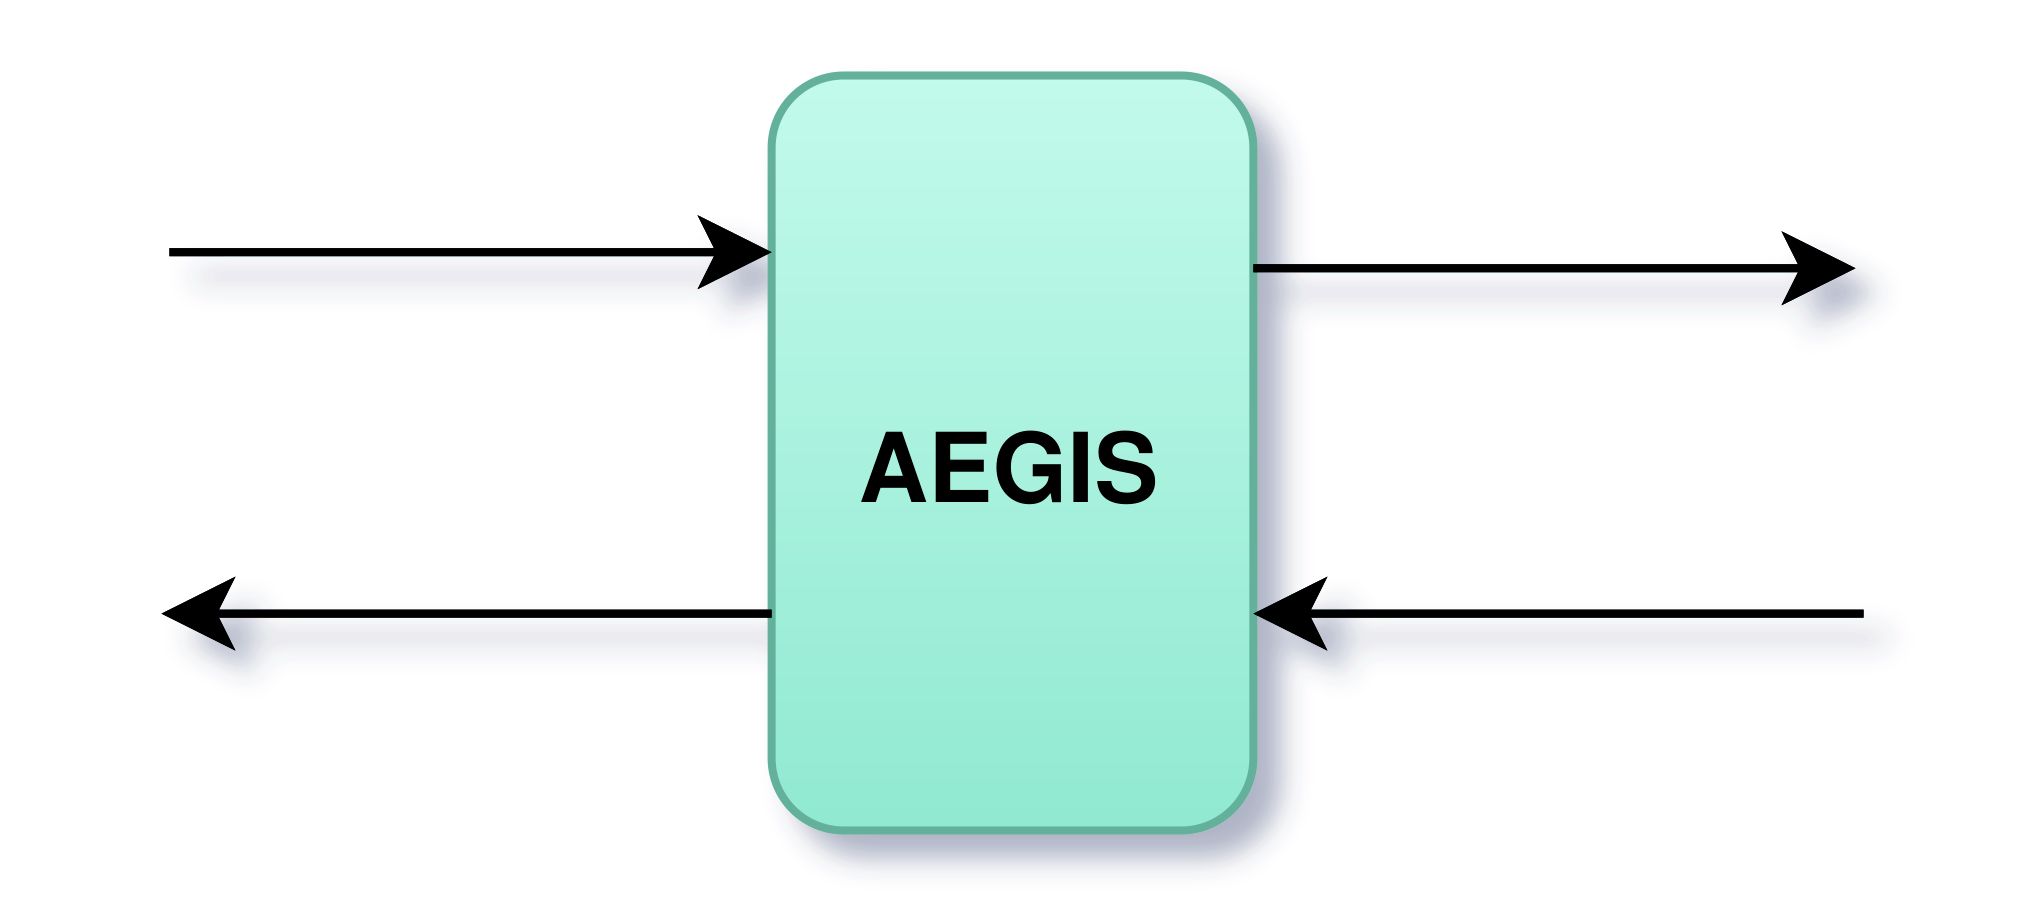
\includegraphics[width=\textwidth]{done/done1.png}
            Pakete weiterleiten
        \end{minipage}
        \begin{minipage}[h]{0.25\textwidth}
            \center
            %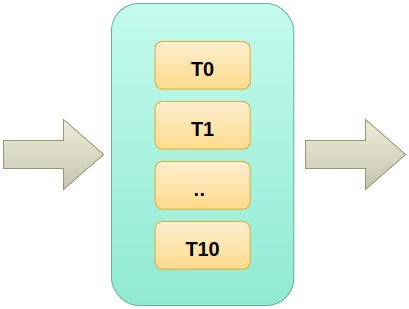
\includegraphics[width=\textwidth]{done/done2.pdf}
            Multithreading
        \end{minipage}
    \end{minipage}
    \vspace{0.5cm}
    \begin{minipage}[h]{\textwidth}
        \center
        \begin{minipage}[h]{0.3\textwidth}
            \center
            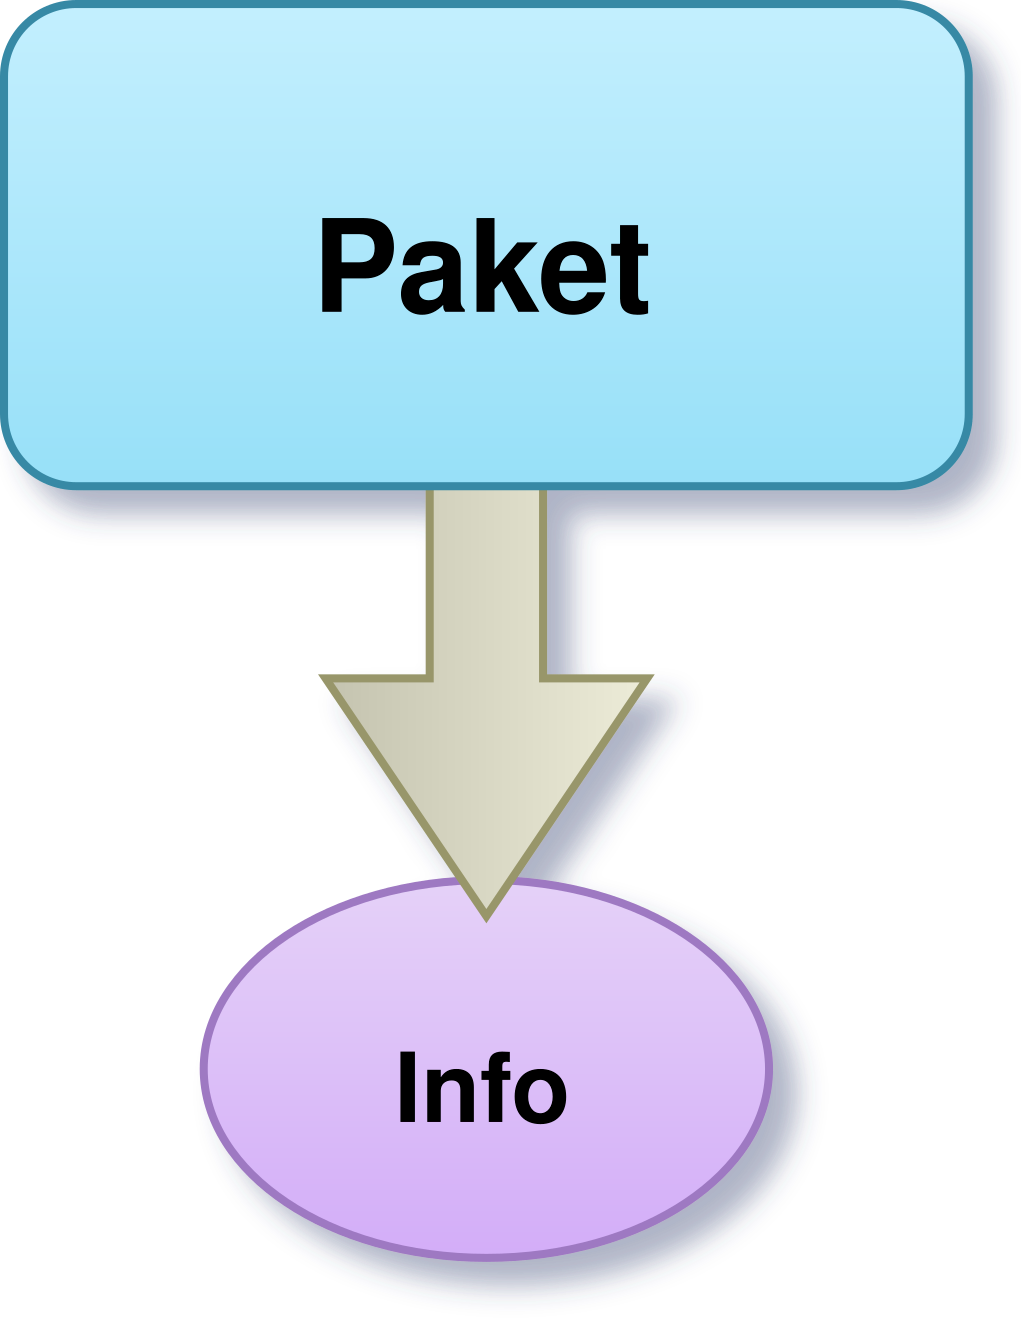
\includegraphics[width=0.5\textwidth]{done/done3.png}
            Informationen aus Paketen extrahieren
        \end{minipage}
    \end{minipage}
\end{frame}

\begin{frame}{Ausblick}
    \begin{itemize}
        \item Anforderungen unverändert
        \item Überprüfung wichtiger Anforderung
        \item Erweiterung um Angriffe und ihre Abwehrmechanismen
    \end{itemize}
\end{frame}

\begin{frame}{Bildquellen}
    \begin{itemize}
        \tiny
        \item https://www.onlinewebfonts.com/icon/571002 [Abgerufen am 22.06.2021]
    \end{itemize}
\end{frame}

\begin{frame}
    \begin{center}
        \textbf{Vielen Dank für Ihre Aufmerksamkeit!}
    \end{center}
\end{frame}

\end{document}